
\documentclass{beamer}
\usetheme{Wrexham}  
\usepackage{graphicx}
\usepackage{color}
\usepackage{caption}
\usepackage{subcaption}
\graphicspath{{./figures/}}
\begin{document}
\title{The Futurama Theorem.}
\subtitle{A friendly introduction to permutations.}
\author{Rhian Davies}
\titlegraphic{ \includegraphics[height=0.5cm]{ri-logo.png} \hspace{3cm} \includegraphics[height=0.8cm]{mathsandstatswhite.jpg}}
%\titlegraphic{\includegraphics[height=.2\textheight]{logoEPSRC.png}}
\date{1\textsuperscript{st} March 2014}

\begin{frame}[plain] 
  \titlepage
\end{frame}

\begin{frame}
  \frametitle{Permutations}
In this class we are going to consider the theory of permutations, and use them to solve a problem posed in an episode of Futurama. 

%A permutation of a set $X$ is a rearrangement of its elements.

\end{frame}

%\begin{frame}
%  \frametitle{Crystallography}
%  \begin{figure}[h]
%    \centering
%    \includegraphics[width = 9cm]{gallium.jpg}
%\caption{``gallium_Crystals.jpg by foobar  Wikimedia Commons  CC BY-SA 3.0''}
%  \end{figure}
%\end{frame}


%\begin{frame}
%  \frametitle{Solving a Rubix Cube}
%  \begin{figure}[h]
%    \centering
    
%\includegraphics[width = 5cm]{rubix.png}
%  \end{figure}


%FACT: There are 43,252,003,274,489,856,000 permutations that can be made of the little
%coloured squares on the faces of Rubik’s cube.

%FACT: Any scrambled Rubik’s cube can, in theory, be restored to its original
%configuration in 20 moves or less.

%\end{frame}

%\begin{frame}
%  \frametitle{Comedy T.V. shows}
%  \begin{figure}[h]
%    \centering
%    \includegraphics[width = 9cm]{futurama.png}
%  \end{figure}
%\end{frame}

\begin{frame}
  \frametitle{What is a permutation?}
A permutation of a set X is a rearrangement of its elements. \\
\textcolor{white}{.}\\
Example\\
Let X =$ \left \{\mbox{Jack, Queen, King} \right\} $. Then there are six permutations: 


Jack Queen King, \qquad Queen King Jack, \qquad King Jack Queen, 

Queen Jack King, \qquad King Queen Jack, \qquad Jack King Queen.
  

%Order is important. 
\end{frame}

%\begin{frame}
%  \frametitle{More precisely...}
%  Definition


%Notation
%Let $X= \left\{1,2, \hdots, n\right\}$ and $\alpha: X \rightarrow X$ be a permutation. It is convienient to describe this function in the following way:


%\[ \alpha = \left( \begin{array}{cccc}
%1 & 2 & \hdots & n  \\
%\alpha(1) & \alpha(2) & \hdots & \alpha(n)  \end{array} \right)   \] 

%\end{frame}

\begin{frame}
  \frametitle{Another example}
%A permutation of a set X is a one-to-one correspondence from X to itself. 
  \begin{itemize}
  \item Let the set be $X = \left \{1,2,3 \right\}$.
    \item Define $\alpha$ be a permutation that takes $\alpha(1) \rightarrow 2, \alpha(2) \rightarrow 3, \alpha(3) \rightarrow 1.$ 
      \item We can think of $\alpha$ as a function machine. 
  \end{itemize}


%So we write:

%\[ \alpha = \left( \begin{array}{cccc}
%1 & 2 &3   \\
%2 & 3 &1  \end{array} \right).   \] 

%Again, let the set be $X = \left \{1,2,3 \right\}$.
%
%Let $\alpha$ be the permutation that takes $\alpha(1) \rightarrow 2, \alpha(2) \rightarrow 3, \alpha(3) \rightarrow 1.$ 

%$\alpha = $   \includegraphics[width = 2cm]{permutation.png}


\begin{figure}[h]
  \centering
  \includegraphics[width = 3cm]{function}
\end{figure}

\end{frame}

\begin{frame}
  \frametitle{Permutation Diagrams}
  We can write this permutation down in a permutation diagram as shown. 

\begin{figure}[h]
  \centering
  \includegraphics[width = 3cm]{permutation}
\end{figure}

$\alpha(1) \rightarrow 2,\qquad \alpha(2) \rightarrow 3,\qquad \alpha(3) \rightarrow 1.$ 

\end{frame}

\begin{frame}
  \frametitle{Lets try multiplying}
  
If we write $\alpha \circ \beta$, this means apply the permutation $\beta$ to our set, and then apply the permutation $\alpha$ to our set. 
We're using the convention working from right to left which might look a bit strange but you'll get used to it.% ($\alpha \circ \beta  = \alpha (\beta (X))$)

Example

\begin{figure}[h]
  \centering
  
  \includegraphics[width = 3cm]{definition.png}
\end{figure}

$\alpha \circ \beta = $

\begin{figure}[h]
  \centering
  
\includegraphics[width= 5cm]{multiply.png}
\end{figure}
\end{frame}

%%%%%%%%%%%%%%%%%%%%%%%%%%%%%%%%%%%%%%%%%%%%%%%%%%%%%%%%%%%%%%%%%%%%%%%%%%%%%%%%%%%%%%%%%%%%%%%%%%%%%%%%%%%%%%%%%%%%%%%%%%%%%%%%%%%%%

%WORKSHEET 1

%%%%%%%%%%%%%%%%%%%%%%%%%%%%%%%%%%%%%%%%%%%%%%%%%%%%%%%%%%%%%%%%%%%%%%%%%%%%%%%%%%%%%%%%%%%%%%%%%%%%%%%%%%%%%%%%%%%%%%%%%%%%%%%%%%%%%


%\begin{frame}
%  \frametitle{Worksheet 1}%
%
%\[ \alpha \circ \beta = \left( \begin{array}{cccc}
%1 & 2 & 3 & 4  \\
%1 & 3 & 2 & 4  \end{array} \right)   \] 
%
%\[ \beta \circ \alpha = \left( \begin{array}{cccc}
%1 & 2 & 3 & 4  \\
%1 & 2 & 4 & 3  \end{array} \right)   \] 
%
%\begin{equation*}
%\alpha \circ \beta \neq \beta \circ \alpha   
%\end{equation*}


%Note: These are not the same. Therefore products of permutations don't necessarily commute.

%\end{frame}

%A diagram that swaps just two elements is called a transposition

%Disjoint transpotitions commute.

%Every permutation can be written as the product of some sequence of transpotions. 

\begin{frame}
  \frametitle{Cycle Notation}
%Mathematicians are lazy so writing out long diagrams is not hand. 
Cycle notation allows us to write down permutation diagrams in a more efficient way.
Lets think about this permutation $\alpha = $ \includegraphics[width = 2.5cm]{c1}
%\[  \alpha = \left( \begin{array}{ccccc}
%1 & 2 & 3 & 4 & 5  \\
%2 & 3 & 4 & 5 & 1  \end{array} \right) .   \] 

We could write this in a cycle, 

\begin{figure}[h]
  \centering
  \includegraphics[height = 2.5cm]{cycleNotation.png}
\end{figure}

or in short hand $\alpha = (1 \; 2 \; 3 \; 4 \; 5)$.




  
\end{frame}

\begin{frame}
  \frametitle{Composition of cycles}
We can write down compositions of cycles without the $\circ$ symbol (again mathematicians are lazy!)

So
\begin{equation*}
   (1 \; 2 \; 3) \circ (4 \; 5) = (1 \; 2 \; 3)(4 \; 5)
\end{equation*}

Example

\begin{equation*}
  (2 \; 3 \; 5)(1 \; 5 \; 4) = (1 \; 2 \; 3 \; 5 \; 4)
\end{equation*}


\textit{Reminder: We work from right to left.}
\end{frame}

\begin{frame}
  \frametitle{Disjoint cycles}
  \begin{itemize}
  \item Two cycles are said to be \textit{disjoint} if they act on disjoint sets of symbols. 

\item In the examples on the previous slide the cycles (1 2 3) \& (4 5) are disjoint, while the cycles (1 5 4) \& (2 3 5) are not.

\item Note  that (1 2 3)(4 5) = (4 5)(1 2 3). These cycles commute. 

\item This makes sense if we look at a diagram.
  \end{itemize}


\end{frame}
\begin{frame}
  \frametitle{Disjoint cycles}
   Since the cycles (1 2 3) and (4 5) are disjoint, they act in a sense independently of one another so it doesn't matter which one you consider to be taking first.

\begin{figure}[h]
  \centering
  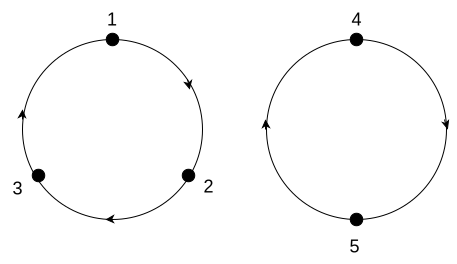
\includegraphics[width =5cm]{disjoint.png}
\end{figure} 
 It is very useful to be able to express a permutation as a product of disjoint cycles, because then its structure is immediately clear. 
\end{frame}



\begin{frame}
  \frametitle{Disjoint cycles: Example}
We write the permutation $\alpha = $ \includegraphics[width=3cm]{c2}
%\[  \alpha = \left( \begin{array}{cccccc}
%1 & 2 & 3 & 4 & 5 & 6  \\
%2 & 5 & 6 & 3 & 1 & 4 \end{array} \right) ,   \] 

as a product of disjoint cycles. 

Start with any number, say 1. Notice that 
\begin{equation*}
  \label{eq:1}
  \alpha: 1 \mapsto 2, \quad 2 \mapsto 5,\quad 5 \mapsto 1. 
\end{equation*}

Thus (1 2 5) is one of the cycles of which $\alpha$ is composed.

Next take any of the remaining numbers, say 3. Then

\begin{equation*}
  \alpha: 3 \mapsto 6,\quad 6 \mapsto 4,\quad 4 \mapsto  3.
\end{equation*}

Hence $\alpha = (1 \; 2 \; 5)(3 \; 6 \; 4) = (3 \; 6 \; 4)(1 \; 2 \; 5).$

\end{frame}

\begin{frame}
  \frametitle{Transpositions}


  \begin{itemize}
  \item A transposition is simply a permutation that only switches 2 elements of the set, and everything else stays the same. 

\item One example of a transposition is (3 4).
  \end{itemize}
  
\end{frame}

%\begin{frame}
 
% So we can express every permutation as a product of disjoint cycles - useful.

%Something else which will be useful later is a 2-cycle of a transposition. 

%Every cycle can be expressed a product of transpositions.*Question* (Not  necessarily disjoint). 




%\end{frame}



%%%%%%%%%%%%%%%%%%%%%%%%%%%%%%%%%%%%%%%%%%%%%%%%%%%%%%%%%%%%%%%%%%%%%%%%%%%%%%%%%%%%%%%%%%%%%%%%%%%%%%%%%%%%%%%%%%%%%%%%%%%%%%%%%%%%%

%WORKSHEET 2

%%%%%%%%%%%%%%%%%%%%%%%%%%%%%%%%%%%%%%%%%%%%%%%%%%%%%%%%%%%%%%%%%%%%%%%%%%%%%%%%%%%%%%%%%%%%%%%%%%%%%%%%%%%%%%%%%%%%%%%%%%%%%%%%%%%%%




%%%%%%%%%%%%%%%%%%%%%%%%%%%%%%%%%%%%%%%%%%%%%%%%%%%%%%%%%%%%%%%%%%%%%%%%%%%%%%%%%%%%%%%%%%%%%%%%%%%%%%%%%%%%%%%%%%%%%%%%%%%%%%%%%%%%%

%BREAK

%%%%%%%%%%%%%%%%%%%%%%%%%%%%%%%%%%%%%%%%%%%%%%%%%%%%%%%%%%%%%%%%%%%%%%%%%%%%%%%%%%%%%%%%%%%%%%%%%%%%%%%%%%%%%%%%%%%%%%%%%%%%%%%%%%%%%

\begin{frame}
  \frametitle{Futurama}

\begin{figure}
        \centering
        \begin{subfigure}[b]{0.25\textwidth}
                \includegraphics[width=\textwidth]{promoFry}
                %\caption{A gull}
                \label{fig:gull}
        \end{subfigure}%
        ~ %add desired spacing between images, e. g. ~, \quad, \qquad etc.
          %(or a blank line to force the subfigure onto a new line)
        \begin{subfigure}[b]{0.25\textwidth}
                \includegraphics[width=\textwidth]{futbook}
                %\caption{A tiger}
                \label{fig:tiger}
        \end{subfigure}
 \end{figure}

%I Love futurama
%American Simpson created by Matt Groening
%Fry from NY pizza delivery
%Maths is everywhere in it - see this clip. 
\end{frame}


\begin{frame}
  \frametitle{The Prisoner of Bender (6x10)}

 % \begin{itemize}
  %\item Professor Farnsworth and Amy build a mind-switching machine.
  %  \item After two bodies have swapped minds, those bodies can't switch minds again.
   % \item During the episode lots of the charecters use the machine - it gets very mixed up.
%\item Eventually they want to return to their original bodies. 
  %     \end{itemize}

  \begin{figure}[h]
    \centering
    \includegraphics[width = 8cm]{mind_switcher.jpg}
  \end{figure}
%Watch another clip
 \end{frame}

 \begin{frame}
 \frametitle{Ken Keeler}

\begin{figure}
        \centering
        \begin{subfigure}[b]{0.3\textwidth}
                \includegraphics[width=\textwidth]{Ken_Keeler}
                %\caption{A gull}
                \label{fig:gull}
        \end{subfigure}%
        ~ %add desired spacing between images, e. g. ~, \quad, \qquad etc.
          %(or a blank line to force the subfigure onto a new line)
        \begin{subfigure}[b]{0.54\textwidth}
                \includegraphics[width=\textwidth]{theorem}
                %\caption{A tiger}
                \label{fig:tiger}
        \end{subfigure}
 \end{figure}

  
 \end{frame}
%The Simpsons and Futuramahe proved a theorem which appears in the Futurama episode "The Prisoner of Benda".[1]
% Ph.D. in applied mathematics from Harvard

\begin{frame}
  \frametitle{Mind swaps}
  \begin{itemize}
  \item Amy $\leftrightarrow$ Professor 
    \item Amy $\leftrightarrow$ Bender
      \item Leela $\leftrightarrow$ Professor
        \item Amy $\leftrightarrow$ Wash Bucket
          \item Fry $\leftrightarrow$ Zoidberg
            \item Emperor Nikolai $\leftrightarrow$ Wash Bucket
              \item Hermes $\leftrightarrow$ Leela
  \end{itemize}

We can write this as a product of transpositions, working right to left.  
(h\;l)(e\;w)(f\;z)(a\;w)(l\;p)(a\;b)(a\;p) 

Task: Write this down in disjoint cycles.
%Amy's Body swaps with Professor's Body
\end{frame}

\begin{frame}
  \frametitle{Challenge.}
  
  \begin{itemize}
  \item Apply the same swaps that happen in the episode.
    \item Try to swap the bodies around to get everyone back to the right place. 
      \item Make sure someone in your group keeps track of the swaps
        \item Remember no pair of bodies can swap more than once. 
          \item Write down the bodies that swap. 
  \end{itemize}
\end{frame}

\begin{frame}
  \frametitle{Fixing a 7-cycle}
  \begin{itemize}
  \item   Consider just the 7-cycle $(1\;2\;3\;4\;5\;6\;7)$.
\item  Introduce two new bodies that have not had their minds swapped, say $x$ and $y$.
\item  To return all minds of back to the right bodies, apply the following sequence of transpositions:
\item $(x\;7)(y\;1)(y\;2)(y\;3)(y\;4)(y\;5)(y\;6)(y\;7)(x\;1)$.
  \end{itemize}
\end{frame}

  \begin{frame}
    \frametitle{Does this work?}


    \begin{itemize}
    \item $(x\;7)(y\;1)(y\;2)(y\;3)(y\;4)(y\;5)(y\;6)(y\;7)(x\;1)(1\;2\;3\;4\;5\;6\;7)=?$

\item Have we swapped the same two bodies more than once?

    \end{itemize}


\end{frame}

\begin{frame}
  \frametitle{What if the cycle is really long?}

  \begin{itemize}
  \item   Consider the k-cycle $(1\;2\; \hdots \;k)$.
    \item Introduce two new bodies that have not had their minds swapped, say x and y.
      \item Apply the following transpositions:        \item $(x\;k)(y\;1)(y\;2)\hdots(y\;k-1)(y\;k)(x\;1)$.
  \end{itemize}

\end{frame}

\begin{frame}
  \frametitle{Why does it work ?   $(x\;k)(y\;1)(y\;2)\hdots(y\;k-1)(y\;k)(x\;1)$.}
 
  \begin{itemize}

\item First step is to apply $(y\;k)(x\;1)$.
\item $(y\;k)(x\;1)(1\;2\; \ldots\; k) = (1\;2\;\hdots\;k-1 \;y\;k\;x)$.
  \item	Then $(y\;k-1)$ puts the mind of $k-1$ back where it belongs.
\item	And then $(y\;k-2)$ puts the mind of $k-2$ back where it belongs.
\item	Continue this until $(y\;1)$ puts the mind of 1 back where it belongs.
\item	And finally, we swap $x$ and $k$.
\item	When we finish $x$ and $y$ are still muddled but they have never swapped with each other!

  \end{itemize}


\end{frame}



\begin{frame}
  \frametitle{Fixing products of disjoint cycles}
  \begin{itemize}
  \item What do we do when we have multiple cycles to start with?
  \item	Use x and y to fix each individual cycle.
  \end{itemize}

%\item	When doing this, x and y will sometimes be swapped.
%\item	If there is an even number of disjoint cycles, then we're done after we fix each individual cycle.
%\item	If there is an odd number of disjoint cycles, then after fixing each individual cycle, finish by swapping x and y.
\end{frame}

%%%%%%%%%%%%%%%%%%%%%%%%%%%%%%%%%%%%%%%%%%%%%%%%%%%%%%%%%%%%%%%%%%%%%%%%%%%%%%%%%%%%%%%%%%%%%%%%%%%%%%%%%%%%%%%%%%%%%%%%%%%%%%%%%%%%%

%ACTIVITY



%%%%%%%%%%%%%%%%%%%%%%%%%%%%%%%%%%%%%%%%%%%%%%%%%%%%%%%%%%%%%%%%%%%%%%%%%%%%%%%%%%%%%%%%%%%%%%%%%%%%%%%%%%%%%%%%%%%%%%%%%%%%%%%%%%%%%



%%%%%%%%%%%%%%%%%%%%%%%%%%%%%%%%%%%%%%%%%%%%%%%%%%%%%%%%%%%%%%%%%%%%%%%%%%%%%%%%%%%%%%%%%%%%%%%%%%%%%%%%%%%%%%%%%%%%%%%%%%%%%%%%%%%%%

%WORKSHEET 3

%%%%%%%%%%%%%%%%%%%%%%%%%%%%%%%%%%%%%%%%%%%%%%%%%%%%%%%%%%%%%%%%%%%%%%%%%%%%%%%%%%%%%%%%%%%%%%%%%%%%%%%%%%%%%%%%%%%%%%%%%%%%%%%%%%%%%


\begin{frame}
  \frametitle{Let's have a go}

  \begin{enumerate}
  \item   Choose two people to be the ``X'' and ``Y'' and label them. 
    \item  Everyone else labels themselves and shuffles their brains.
      \item  Everyone (except X and Y) stand so the \textbf{person on your left holds your brain}.
        \item  Make your (disjoint) cycles into long lines. 
          \item Fix each cycle, one at a time.
            \begin{itemize}
             \item  X swaps with person with no-one on their \textbf{right hand side}.
            \item  Y swaps with person with no-one on their \textbf{left hand side}.
              \item Y continues to swap with everybody people down the line (except X). 
              \item Swap the mind in X's body back where it belongs, into the body at the back of the line. 
            \end{itemize}
                         \item Once all cycles are fixed, swap the two helpers (if necessary).
  \end{enumerate}

 

\end{frame}


\begin{frame}
  \frametitle{Questions for the road.}
  \begin{itemize}
  \item In which situations do we need to need to swap X and Y at the end?
\item What is the minimum number of switches required?
  \end{itemize}

More info at \url{www.lancs.ac.uk/~daviesr3/rimasterclass}
\end{frame}

% Other questions, 

%When will we need the helpers to swap bodies?
%

\end{document}